\documentclass[11pt]{article}
\usepackage[margin=1.1in]{geometry}
\usepackage{amsmath,amssymb}
\usepackage{booktabs}
\usepackage{graphicx}
\usepackage{natbib}
\usepackage[hidelinks]{hyperref}
\usepackage{xcolor}
\usepackage{microtype}
\newcommand{\qwen}{Qwen3.5-2B}

\title{The Lifelong Loop: Error-Gated Consolidation\\ and the Cost of Nights Without a Log}
\author{Xuhao Lin\\ \small Independent researcher \quad \texttt{linxuhao84@gmail.com}}
\date{July 2026 --- v1.1 (preprint)}

\begin{document}
\maketitle

\begin{abstract}
Can an agent whose long-term memory lives in the weights of a frozen language model keep learning,
day after day? We run a complete day/night memory loop end-to-end for up to 30 simulated days (720
facts): each day streams facts into a disposable LoRA ``day'' adapter with error-gated writes; each
night consolidates into a persistent ``core'' adapter and resets the day store; after every night,
per-fact recall and 2-AFC recognition are probed over the \emph{entire} history. Five findings, all
with a capability firewall (adapter-off equals base) intact in every run. (1)~At \emph{identical}
nightly budget, \textbf{error-gated consolidation} --- train the core only on what it currently
fails --- retains $2.2\times$ more than recency-only consolidation and flattens the retention-by-age
curve. (2)~The class that untargeted consolidation loses is precisely the \emph{latent} one: facts
recognized-but-not-recalled have 0\% next-day survival under recency-only consolidation (0/588) and
46\% under error-gating --- above even the recalled class, because the miss list targets them.
(3)~\textbf{Nights without a log do not merely fail; they poison}: pure self-recitation collapses
structurally (0/144 --- the core cannot recite what only the day adapter learned), and mixing
recitation with ground truth is \emph{worse than doing nothing about the past} (4.3/144, below the
recency baseline's 25.0), because wrongly-recited old facts overwrite earlier consolidation ---
error compounding, a within-system analogue of model collapse. (4)~Over a 30-day horizon at fixed
budget, \textbf{neither anticipated exhaustion occurs}: full replay holds 99\% of 720 facts (the r32
core's streaming capacity exceeds the stream our generator can produce), and the error-gated arm's
retained \emph{fraction} rises with horizon (38\% $\to$ 44\% $\to$ 46\%), settling into a throttled
steady state --- a stable old-day plateau bought by squeezing intake of the newest days.
(5)~The served agent is \textbf{not aphasic} --- GSM8K is intact with adapters mounted in both
serving states --- but free-text fluency shows a graded, super-additive ``accent'' that concentrates
in the hot-day serving state, the same state responsible for a $3$--$10\times$ \emph{read-time
masking} of old facts. Together these results yield a concrete design rule for log-backed,
self-testing in-weight memory: consolidate nightly on failures, serve from the core, mount the day
adapter narrowly --- and never let the system rehearse its own unverified recall.
\end{abstract}

\section{Introduction}

Deployed LLM agents accumulate experience, but their weights do not: memory is delegated to context
windows, retrieval stores, and files, while the model itself stays frozen. A growing line of work
proposes to close that gap with a sleep-like loop --- act during the day, consolidate into parameters
at night \citep{letThemSleep2026,scm2026,behrouz2024titans}. The proposals are architectural; what
the field lacks is \emph{measurement}: when such a loop actually runs for many days, what survives,
what is lost, what does each night's policy cost, and does the host model remain usable?

In companion work \citep{lin2026persistence} we audited the \emph{day} scale: single-pass fact
streams written into a LoRA adapter on a frozen base, instrumented per fact. Three results from that
audit drive the present design. First, online in-weight memory accumulates by
\emph{re-instatement}, not persistence --- capacity is determined by what gets re-trained after it
slips, so the schedule of re-instatement is the central design variable. Second, forgetting under
protected writes is largely \emph{suppression} rather than erasure: a cheap two-alternative
recognition probe shows most ``forgotten'' facts remain latent, which makes targeted re-instatement
cheap. Third, spending a fixed replay budget on \emph{self-test failures} converts those latent
facts back to expressed ones at no extra cost.

This paper closes the loop. We run a complete day/night system --- disposable day adapter, persistent
core, ground-truth log, nightly consolidation, daily reset --- for 6, 12, and 30 simulated days, and
we treat the night policy as the experimental variable under a fixed gradient budget. The questions
are the ones a lifelong-learning deployment would actually face: Should the night replay everything
(cost grows without bound), only the most recent day (cheap, but what of the past?), only what the
core currently fails (cheap and targeted, but the failure list grows), or the core's own recitations
(no log dependency at all)? What breaks first as the horizon grows --- the budget, or the core's
capacity? And is the agent still a usable language model while all of this is mounted?

\paragraph{Contributions.}
\begin{enumerate}
\item \textbf{An end-to-end loop instrument} (\S\ref{sec:instrument}): per-fact recall and
recognition over the entire history after every night, retention-by-age curves, category-conditioned
survival (recalled / latent / gone), dual-state capability probes, and a capability firewall checked
in every run --- to our knowledge the first per-fact audit of a multi-day consolidate-into-weights
loop.
\item \textbf{Budget-matched night policies} (\S\ref{sec:policies}): error-gated consolidation
retains $2.2\times$ recency-only consolidation at identical budget (55.3 vs.\ 25.0 of 144) and
flattens the age curve; the mechanism is located in the \emph{latent} class, whose next-day survival
is 0\% without targeting and 46\% with it.
\item \textbf{The log is load-bearing --- twice} (\S\ref{sec:nolog}): in a day/core split the core
cannot recite what only the day adapter learned (pure self-recitation: 0/144), and it cannot
\emph{safely} recite what it partially learned: a pre-registered hybrid (recite old + log for today)
landed \emph{below} the recency baseline (4.3 vs.\ 25.0) because wrong recitations actively
overwrite earlier consolidation. Active wrong-value rehearsal is worse than passive decay.
\item \textbf{Horizon behavior at fixed budget} (\S\ref{sec:horizon}): across 6 $\to$ 12 $\to$ 30
days (144 $\to$ 720 facts), the error-gated arm's retained fraction \emph{rises} (38/44/46\%) and
settles into a throttled steady state (old-day plateau, squeezed intake); full replay holds 99\% at
720 facts, so the r32 core's streaming capacity exceeds what our fact generator can produce. Neither
the pre-registered budget collapse nor capacity exhaustion occurs; both knees lie beyond this toy's
reach.
\item \textbf{Dual-state capability and read-time masking} (\S\ref{sec:capability}): mounted
adapters leave GSM8K intact in both serving states (no task-level aphasia), but free-text NLL rises
super-additively under the hot day mount ($\sim$6$\times$ perplexity), and the same state masks old-fact
recall $3$--$10\times$ at read time. The serving prescription follows: consolidate nightly, serve
from the core, mount the day adapter narrowly.
\end{enumerate}

As in the companion paper, everything is reported as floors and directions --- synthetic facts,
1--3 seeds per condition on nondeterministic consumer hardware --- with per-seed numbers throughout
and raw per-fact timelines released. The six-day, five-arm comparison replicates structurally on a
second substrate (\S\ref{sec:transfer}); the longer horizons are single-substrate.

\section{Related work}\label{sec:related}

\textbf{Sleep-cycle agents.} Architectures that batch daytime experience and consolidate into
parameters at rest are now numerous --- adaptive agents with sleep phases
\citep{letThemSleep2026}, sleep-consolidated memory \citep{scm2026}, and test-time memorization
lines \citep{behrouz2024titans}. These works build and assert; we instrument and measure a running
loop per fact, per night, per age --- and several of their implicit assumptions (that self-distillation
suffices; that serving with all adapters mounted is free) fail measurably here.
\textbf{Complementary learning systems.} The day/core split follows CLS \citep{mcclelland1995}:
a fast, disposable store and a slow, protected one, with consolidation between. Our results give the
computational version two sharp caveats: consolidation must be driven by ground truth (not replayed
dreams of it), and the fast store interferes with the slow one at \emph{read} time, not just write
time. \textbf{Replay and selection.} Prioritized and interference-aware replay
\citep{schaul2015,aljundi2019mir}, surprise-gated storage \citep{sure2025}, and forgetting-curve
schedules \citep{mssr2026} motivate the error-gated night; as in the companion paper we claim no
novelty for the selection rule itself --- the contribution is the budget-matched measurement of what
it buys (and what its self-test costs) inside a full loop. Pseudo-rehearsal \citep{robins1995}
anticipated consolidation without stored data; our recite and hybrid arms are its LLM-scale test,
and they fail in an instructive way: generation quality is now high enough that wrong recitations
are \emph{fluent}, so they train as effectively as truth --- which is precisely the problem. The
collapse dynamics echo training-on-own-outputs degradation \citep{shumailov2024} inside a single
system. \textbf{Behavioral horizon scaling.} Long-horizon environment learning now has behavioral
scaling laws \citep{edgebench2026}; the substrate-level question underneath --- what happens to
in-weight memory as the horizon grows --- is the gap this paper measures.

\section{The loop instrument}\label{sec:instrument}

Frozen \qwen{} base (fp32, eager attention); persistent rank-32 \textsc{core} adapter + disposable
rank-64 \textsc{day} adapter (both all-linear LoRA, $\alpha{=}2r$; AdamW, lr $3{\times}10^{-5}$).
Facts are collision-free \emph{``The user's \{attribute\} is \{pseudoword\}.''} statements
\citep[the day-scale instrument of][]{lin2026persistence}; 24 facts per day.

\textbf{Day.} Each fact: 8 value-masked write steps into \textsc{day} with summed-Fisher EWC
($\lambda{=}300$), plus 4 replay steps spent on the most recent self-test's failures (the day-scale
winner). Serving state during the day: \textsc{core+day}.

\textbf{Night.} Consolidate into \textsc{core}, then delete and re-initialize \textsc{day}. The
gradient budget is fixed at $72 = 24\times3$ steps per night for every arm except \emph{full}:
\begin{itemize}
\item \emph{full}: all past true statements, 3 epochs --- budget grows with history; the reference
ceiling, deliberately \textbf{not} budget-matched;
\item \emph{markov}: today's true statements only --- the scalable recency baseline;
\item \emph{misslog}: probe \textsc{core}-alone recall over the whole history (the mechanism's
self-test; a generation cost that grows linearly with history, not a gradient cost), then train only
on current failures, from the log;
\item \emph{recite}: self-distill the core's own greedy completions of the whole history --- no log;
\item \emph{hybrid}: today from the log + old facts self-recited, budget spread uniformly.
\end{itemize}

\textbf{Probes.} After every night (every third night at the 30-day horizon), \textsc{core}-only
greedy recall and 2-AFC recognition margins over \emph{all} facts so far; the distractor for each
fact is another fact's value from the same stream, so a positive margin measures fact-specific
binding. \textbf{Firewall}: GSM8K (10-item fixed subset) with all adapters disabled, before and
after every run. \textbf{Dual-state capability} (\S\ref{sec:capability}): GSM8K and fixed-text
NLL/token with \textsc{core+day} mounted (end of day) and \textsc{core} alone (after night).
Seeds 1234/2025/777 (D6), 1234/2025 or 1234 (D30); consumer ROCm GPUs are nondeterministic at fixed
seed, so all numbers are directions with per-seed values shown. Fact cohorts at equal seed are
prefix-identical across horizons, so D6/D12/D30 comparisons are exact.

\section{Results}

\subsection{Night policy at matched budget}\label{sec:policies}

\begin{table}[t]\centering\small
\begin{tabular}{lcccc}
\toprule
night arm & final recall /144 (seeds) & mean & final recognition /144 & next-day survival R/L/G \\
\midrule
full (ceiling) & 134/142/133 & 136.3 & 144/144/143 & 93\% / 80\% / 67\% \\
misslog        & 52/60/54    & \textbf{55.3} & 117--125 & 36\% / \textbf{46\%} / 30\% \\
markov         & 26/25/24    & 25.0  & 89--107  & 14\% / \textbf{0\%} / 0\% \\
hybrid         & 6/6/1       & 4.3   & 72--89 ($\approx$chance) & --- \\
recite         & 0/0/0       & 0.0   & 55--76 ($\approx$chance 72) & --- \\
\bottomrule
\end{tabular}
\caption{Six-day loop (144 facts), post-night core-only recall of the full history. R/L/G =
next-day survival of facts that were recalled / latent (recognized-only) / gone at the previous
probe, pooled over seeds and days. Firewall $0.70\to0.70$ in every run.}
\label{tab:d6}
\end{table}

Table~\ref{tab:d6}: at identical nightly budget, error-gated consolidation retains $2.2\times$ the
recency baseline (55.3 vs.\ 25.0 of 144), and the age curves (Fig.~\ref{fig:horizon}a shows the
30-day version) differ in kind: markov keeps only a $\sim$2-day recency window; misslog holds a
plateau across all past days, paid for by lower retention of the newest days.

The survival-by-category columns locate the mechanism. Under markov, facts that were \emph{latent}
--- recognized but not recalled, the suppressed class that dominates in-weight forgetting
\citep{lin2026persistence} --- have \textbf{zero} next-day survival (0/588): each further night of
recency-only training erases precisely the class that was cheapest to save. Under misslog the same
class survives at 46\%, \emph{above} the recalled class (36\%), because the self-test's miss list
preferentially targets it. Error-gated consolidation is, operationally, a latent-fact harvester.

\subsection{Nights without a log: recitation does not just fail, it poisons}\label{sec:nolog}

Pure self-recitation collapses structurally (0/144, recognition at chance): in a day/core split, the
core cannot recite content that only the day adapter learned, so there is nothing meaningful to
distill and the night trains on noise. This is an architectural fact --- single-core designs, where
the core itself day-learns before reciting, degrade far more gracefully --- and it is one half of why
the log is load-bearing.

The \emph{hybrid} arm was pre-registered (2026-07-08) to rescue this: today's facts from the log
(solving the structural problem), old facts recited, same budget --- our prediction placed it between
markov and misslog. \textbf{The prediction was falsified downward: 4.3/144, below markov.} Per-cohort
traces show why. Hybrid's today-cohort consolidates normally at its own night (7/9/4 of 24,
comparable to markov) and is then \emph{erased} over subsequent nights, reaching $\sim$0 by day 6,
while markov's cohorts merely decay passively (19--22 of 24 survive one night). The difference:
hybrid \emph{actively rehearses wrong values}. Each night it recites old clozes mostly incorrectly
--- fluently, plausibly, in exactly the training format --- and gradient descent cannot tell fluent
errors from truth. The errors overwrite earlier correct consolidation and compound across nights: a
within-system analogue of model collapse \citep{shumailov2024}, and the second half of why the log
is load-bearing. \textbf{If ground truth is unavailable for the past, doing nothing about the past
(markov) beats self-distilling it (hybrid) by $6\times$.}

\subsection{Horizon: fixed budget vs.\ growing history}\label{sec:horizon}

\begin{figure}[t]\centering
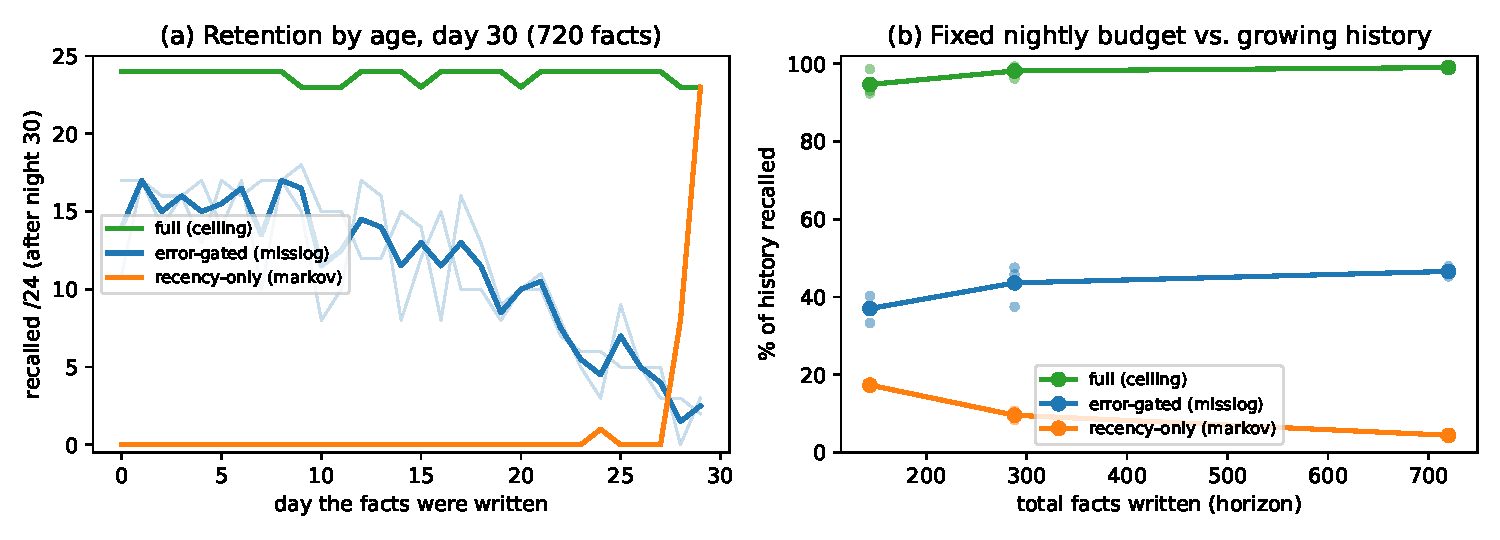
\includegraphics[width=\linewidth]{fig_horizon.pdf}
\caption{(a) Retention by write-day after night 30 (720 facts; thin lines = seeds, thick = mean).
Full replay is flat at ceiling; error-gated consolidation holds an old-day plateau and pays with
throttled intake of the newest days; recency-only keeps a two-day window. (b) Fraction of the whole
history recalled vs.\ horizon at fixed nightly budget: the error-gated fraction \emph{rises}
(38\%$\to$44\%$\to$46\%) while recency-only collapses (17\%$\to$10\%$\to$4\%).}
\label{fig:horizon}
\end{figure}

We pre-registered (2026-07-08) three horizon predictions: (a) full replay stays $\ge$90\% unless the
r32 core saturates; (b) markov keeps a constant absolute window; (c) the error-gated arm's fraction
falls below its 6-day value as the fixed budget races the growing miss list --- with the shape of the
decline as the finding. Outcomes at 12 days (288 facts) and 30 days (720 facts,
Fig.~\ref{fig:horizon}): (a) \emph{held} --- 98\% at 288, \textbf{99\% at 720 (713/720, recognition
720/720, every day at 22--24/24)}: the core's streaming capacity exceeds what our collision-free
generator can produce (784 unique attributes), so the capacity knee is beyond this toy's reach;
(b) \emph{held exactly} --- 32/720 (4.4\%), the last $\sim$2 days; (c) \textbf{falsified in the
favorable direction} --- the error-gated fraction \emph{rose} across horizons (38\% $\to$ 44\% $\to$
45--48\%). The by-day curves show the regime it settles into: an old-day plateau at 8--17/24 with
intake of the newest $\sim$5 days squeezed to 2--6/24. At fixed budget the system does not race to a
cliff; it \textbf{throttles intake to protect its stock} --- a stable steady state in which final
recognition is still 639--646/720 ($\sim$89\%), so the latent pool continues to dwarf expressed
recall even after a month of nights. Locating the true knee requires harsher ratios (more facts per
night-step) or a larger generator; both are future work, and we note plainly that our fact generator
was exhausted before the system was.

\subsection{Is the served agent still functional? Dual-state capability and read-time masking}
\label{sec:capability}

All metrics above are cloze completions; a deployment needs the mounted agent to remain a usable
language model. Re-running the 6-day error-gated arm with capability probes in both serving states
(2 seeds) answers this. \textbf{Structured tasks are intact in both states}: GSM8K is 0.70--1.00
with the core alone (morning state) and 0.70--0.90 with the hot day adapter mounted (daytime state),
vs.\ base 0.70 --- 24/24 measurements at or above base. No task-level aphasia. \textbf{Free-text
fluency shows a graded accent}: NLL/token on fixed neutral text rises from 2.93 (base) to 3.21--3.53
with the core alone --- growing slowly with consolidated days --- and to 4.4--5.0 under the hot day
mount ($\sim$6$\times$ perplexity), super-additively (each adapter alone is mild).

The hot day mount is also the state that damages \emph{memory} readout. Comparing each night's
pre-consolidation probe (\textsc{core+day}) with its post-consolidation probe (\textsc{core} only)
exposes a systematic gap at every horizon in every arm: at the 30-day final night the error-gated
run recalls 70/720 with the hot day adapter attached and 326/720 without it; even full replay shows
678 vs.\ 713. A freshly-written day adapter dominates the readout and emits its own day's values for
old prompts: \textbf{concurrent adapter serving taxes old-fact recall $3$--$10\times$}. Both
pathologies concentrate in one serving state, which yields the deployment prescription:
\emph{consolidate nightly; serve from the core; mount the day adapter narrowly (for
recent-information queries) or attenuated --- not permanently}.

\subsection{Substrate transfer: the ordering is an architecture fact}\label{sec:transfer}

Re-running all five night arms for six days on SmolLM2-1.7B-Instruct --- a different organization,
architecture family, and training corpus, with every hyperparameter carried over unchanged --- was
pre-registered (2026-07-11) to preserve the structural claims but not the magnitudes. All four
held (2 seeds, firewall $0.40\to0.40$ in all ten runs): error-gated consolidation beats recency-only
$2.0\times$ (35.0 vs.\ 17.5 of 144; the Qwen ratio is $2.2\times$); pure recitation collapses
structurally (0/144, recognition at chance); \textbf{hybrid recitation poisons even harder} (0.5/144
--- consistent with the mechanism, since a weaker substrate recites with lower fidelity and so
compounds errors faster); and full replay is a substrate-robust ceiling (136/144, recognition
144/144). The markov recency-window signature ([0,0,0,0,3--4,12--15]) and the hot-mount read-time
masking ($6$--$30\times$ on the error-gated arm) also transfer. The night-policy ordering, the
poisoning, and the recency window are properties of the loop architecture, not accidents of one
model.

\section{Discussion}\label{sec:discussion}

\textbf{A design rule, stated once.} The loop's results compose into a single sentence: a lifelong
in-weight memory should be \emph{log-backed} (recitation poisons), \emph{self-testing} (the latent
class is invisible to recency policies and free to harvest), \emph{error-gated at both timescales}
(day writes and night consolidation), and \emph{served from its slow store} (the fast store taxes
both fluency and old recall at read time). Every clause is a measured comparison, not a preference.
\textbf{What the steady state means.} The throttled regime --- protect the stock, squeeze the intake
--- is not a failure mode; it is what bounded consolidation \emph{should} do, and it mirrors the
classic stability--plasticity trade-off surfacing at the systems level. But it implies a design
obligation: intake throttling must be made visible (the system's newest knowledge is its weakest),
e.g.\ by routing recent-information queries to the day adapter or the log rather than the core.
\textbf{What would falsify the rule.} A consolidation policy that beats misslog at matched budget
without a log (contradicting \S\ref{sec:nolog}), or a horizon at which the throttled state collapses
rather than plateaus (contradicting \S\ref{sec:horizon}), or a substrate where recitation is
high-fidelity enough to avoid poisoning. All three are runnable with the released instrument.

\section{Limitations}\label{sec:limits}

The six-day policy comparison is two-substrate (\S\ref{sec:transfer}); the 12- and 30-day horizons
are \qwen{}-only. Synthetic, collision-free, non-conflicting facts; 24 facts per day is a toy day;
revision (``the user moved'') is untested in the loop. One nightly budget (72 steps) and one
day/core rank pair; the throttled steady state's location presumably moves with both. 1--3 seeds per
condition on nondeterministic hardware --- directions, not calibrated points. The misslog self-test
costs generation time linear in history; a deployment would subsample it, and whether sampled
self-tests preserve the steady state is untested. The hybrid arm spreads its budget uniformly
(today's per-fact share shrinks with history); a weighted variant could soften --- though, per the
cohort traces, not eliminate --- the poisoning. Capability probes are GSM8K (10 items) plus a
fixed-text NLL meter; free-form dialogue quality was not scored. Recognition margins use same-stream
distractors; margins near zero are not calibrated confidence.

\section{Conclusion}

Run end-to-end for a month of simulated days, a frozen-base day/core memory system neither collapsed
nor ran out of room --- but only under a specific discipline: ground truth in the loop every night,
consolidation targeted at what the system itself fails, and serving from the slow store. Relax any
clause and the failure is measurable and mechanistically legible: skip the log and the system
poisons itself with its own fluent errors; skip the targeting and the latent majority of memory dies
silently; serve from the fast store and both fluency and old recall pay multiples. The loop's
economics settle into a throttled steady state --- stock protected, intake squeezed --- whose knee
lies beyond what our toy could reach. The per-fact, per-night instrument is released so that the
knee, the substrates, and the policies we did not test can be measured rather than asserted.

\section*{AI disclosure}
As in the companion paper: Claude Fable~5 and Claude Opus (Anthropic) implemented and ran the
experiments, performed related-work searches, and drafted the manuscript under the author's
direction; research questions, designs, pre-registrations, and final claims were set and approved by
the author; all reported numbers re-derive from the released raw timelines.

\begin{thebibliography}{20}\small

\bibitem[Aljundi et al.(2019)]{aljundi2019mir} Aljundi, R., et al. Online continual learning with
maximally interfered retrieval. \emph{NeurIPS} 2019.

\bibitem[Behrouz et al.(2024)]{behrouz2024titans} Behrouz, A., Zhong, P., \& Mirrokni, V. Titans:
Learning to memorize at test time. arXiv:2501.00663.

\bibitem[ByteDance Seed(2026)]{edgebench2026} ByteDance Seed. EdgeBench: Unveiling scaling laws of
learning from real-world environments. 2026. \url{https://edge-bench.org}.

\bibitem[Hazard et al.(2025)]{sure2025} Hazard, H., Fountas, Z., Benfeghoul, M.~A., Oomerjee, A.,
Wang, J., \& Bou-Ammar, H. SuRe: Surprise-driven prioritised replay for continual LLM learning.
arXiv:2511.22367.

\bibitem[Kirkpatrick et al.(2017)]{kirkpatrick2017} Kirkpatrick, J., et al. Overcoming catastrophic
forgetting in neural networks. \emph{PNAS}, 114(13).

\bibitem[Lin(2026)]{lin2026persistence} Lin, X. Persistence is not accumulation: Erasure,
suppression, and re-instatement in online in-weight memory for language models. Preprint,
doi:10.5281/zenodo.21232648.

\bibitem[Lu et al.(2026)]{mssr2026} Lu, Y., He, Y., Chen, J., \& Zha, H. MSSR: Memory-aware adaptive
replay for continual LLM fine-tuning. arXiv:2603.09892.

\bibitem[McClelland et al.(1995)]{mcclelland1995} McClelland, J.~L., McNaughton, B.~L., \& O'Reilly,
R.~C. Why there are complementary learning systems in the hippocampus and neocortex. \emph{Psych.\
Review}, 102(3).

\bibitem[Robins(1995)]{robins1995} Robins, A. Catastrophic forgetting, rehearsal and pseudorehearsal.
\emph{Connection Science}, 7(2).

\bibitem[Schaul et al.(2015)]{schaul2015} Schaul, T., Quan, J., Antonoglou, I., \& Silver, D.
Prioritized experience replay. \emph{ICLR} 2016.

\bibitem[Shumailov et al.(2024)]{shumailov2024} Shumailov, I., et al. AI models collapse when
trained on recursively generated data. \emph{Nature}, 631.

\bibitem[Sleep-cycle agents(2026)]{letThemSleep2026} Let them sleep: Adaptive LLM agents via a sleep
cycle. 2026.

\bibitem[Sleep-consolidated memory(2026)]{scm2026} SCM: Sleep-consolidated memory for continual LLM
agents. arXiv:2604.20943.

\end{thebibliography}

\appendix
\section{Reproduction}
Driver: \texttt{loop.py} (night arm, days, budget, probe stride, dual-state capability probes,
core checkpointing); raw per-night, per-fact timelines: \texttt{results/loop\_*.json};
\texttt{analyze.py} re-derives every table and \texttt{make\_figure.py} the figure. The day-scale instrument, its results,
and the companion paper are at doi:10.5281/zenodo.21199026. Seeds and hyperparameters as in
\S\ref{sec:instrument}.

\end{document}
